% Chapter 4

\chapter{The one dimensional Fermi Hamiltonian} % Main chapter title

\label{Chapter4} % For referencing the chapter elsewhere, use \ref{Chapter3} 

\lhead{Chapter 4. \emph{1D Fermi Hamiltonian}} % This is for the header on each page - perhaps a shortened title

%----------------------------------------------------------------------------------------
In this chapter we will finally arrive at the promised Kitaev Hamiltonian promised in chapter \ref{Chapter2}. Firstly, we calculate the pair interaction Hamiltonian for the fermions in section \ref{sec.HFFint}. This is done under the assumption, that we can restrict the induced interaction to have a vanishing Matsubara frequency: $\omega_q = 0$. I will make an argument for the validity of this approach in section \ref{sec.RetardationEffects}. The result for the interaction Hamiltonian is then inserted into the full Hamiltonian in section \ref{sec.HFFfull}. 

\section{The fermion interacting Hamiltonian} \label{sec.HFFint}

We start out in real space. The interaction Hamiltonian for pair interactions is given by:
\begin{equation}
H^\text{int}_{FF} = \int dxdx' \hat{\psi}^\dagger_F(x)\hat{\psi}^\dagger_F(x')\tilde{V}^\text{ind}_{FF}(x'-x,0) \hat{\psi}_F(x') \hat{\psi}_F(x).
\label{eq.HFFintdef}
\end{equation}
With $\tilde{V}^\text{ind}_{FF}(x'-x,0)$ being the induced interaction at zero frequency in real space (see equation \eqref{eq.VFFx_exact}). Further we make a mean field approximation to get the Hamiltonian on a solvable quadratic form. We write
\begin{equation}
\hat{\psi}_F(x') \hat{\psi}_F(x) = \langle \hat{\psi}_F(x') \hat{\psi}_F(x) \rangle + \left(\hat{\psi}_F(x') \hat{\psi}_F(x)-\langle \hat{\psi}_F(x') \hat{\psi}_F(x) \rangle \right) = \langle \hat{\psi}_F(x') \hat{\psi}_F(x) \rangle + A_F(x',x)
\end{equation}
and treat the last part $A_F$ as a small quantity. The meaning of this will become clearer later on. The mean in the end has to be taken with respect to the specific state of the system, we will also see how this plays out later on. We now only keep terms of $A_F$ and $A^\dagger_F$ up to first order, so that we get the following three terms for the interaction Hamiltonian:\footnote{Formally we are decoupling the Hamiltonian, so that it so no longer really describing any interaction.}
\begin{align}
H^\text{int}_{FF} = &\int dxdx' \langle \hat{\psi}^\dagger_F(x) \hat{\psi}^\dagger_F(x') \rangle \tilde{V}^\text{ind}_{FF}(x'-x,0) \langle \hat{\psi}_F(x') \hat{\psi}_F(x) \rangle + \nonumber \\
&\int dxdx' A^\dagger_F(x,x') \tilde{V}^\text{ind}_{FF}(x'-x,0) \langle \hat{\psi}_F(x') \hat{\psi}_F(x) \rangle + \nonumber \\
&\int dxdx' \langle \hat{\psi}^\dagger_F(x) \hat{\psi}^\dagger_F(x') \rangle \tilde{V}^\text{ind}_{FF}(x'-x,0) A_F(x',x). \nonumber
\end{align} 
To get back to momentum space we expand the field operators in terms of plane waves: $\hat{\psi}_F(x) = \frac{1}{\sqrt{\mathcal{L}}}\sum_k \text{e}^{ikx} f_k$, where as usual $f_k$ is the fermion annihilation operator. Further we assume, that only states belonging to opposite momenta couples.\footnote{At least they are assumed to be absolutely dominant.} This means, that $f_kf_{k'} = f_kf_{k'}\delta_{k,-k'}$, which is the usual BCS assumption. With this, we get the following expression:
\begin{align}
\hat{\psi}_F(x') \hat{\psi}_F(x) &= \frac{1}{\mathcal{L}}\sum_{k} \text{e}^{ik(x-x')}f_kf_{-k} = \frac{1}{2\mathcal{L}}\sum_{k} \left(\text{e}^{ik(x-x')}f_{k}f_{-k}+\text{e}^{-ik(x-x')}f_{-k}f_{k}\right) \nonumber \\
&= \frac{i}{\mathcal{L}}\sum_{k} \sin(k(x-x'))f_{k}f_{-k}, 
\end{align}
where we in the last equality used, that the operators anticommute. Let us plug this into the first term of the interaction Hamiltonian to see how it plays out: 
\begin{align}
H^\text{int}_{FF,1} &= \int dxdx' \langle \hat{\psi}^\dagger_F(x) \hat{\psi}^\dagger_F(x') \rangle \tilde{V}^\text{ind}_{FF}(x'-x,0) \langle \hat{\psi}_F(x') \hat{\psi}_F(x) \rangle \nonumber \\
&= - \frac{1}{\mathcal{L}^2}\sum_{k,k'}\langle f^\dagger_{k}f^\dagger_{-k} \rangle \langle f_{k'}f_{-k'} \rangle \int dx dx' \sin(k(x'-x))\sin(k'(x'-x))\tilde{V}^\text{ind}_{FF}(x'-x,0) \nonumber \\
&= - \frac{1}{\mathcal{L}}\sum_{k,k'}\langle f^\dagger_{k}f^\dagger_{-k} \rangle \langle f_{k'}f_{-k'} \rangle \int du \sin(ku)\sin(k'u)\tilde{V}^\text{ind}_{FF}(u,0) \nonumber \\
&= - \frac{1}{2\mathcal{L}}\sum_{k,k'}\langle f^\dagger_{k}f^\dagger_{-k} \rangle \langle f_{k'}f_{-k'} \rangle W^\text{ind}_{FF}(k,k')
\end{align}
where we use the substitution $u = x'-x$ and use that $\int dx = \mathcal{L}$. Further we have defined the coupling potential $W^\text{ind}_{FF}(k,k')$. The two last terms are analogous and yield:
\begin{align}
H^\text{int}_{FF,2} &= - \frac{1}{2\mathcal{L}}\sum_{k,k'}\left(f^\dagger_k f^\dagger_{-k} - \langle f^\dagger_k f^\dagger_{-k}\rangle\right)\langle f_{k'}f_{-k'} \rangle W^\text{ind}_{FF}(k,k'), \nonumber \\
H^\text{int}_{FF,3} &= - \frac{1}{2\mathcal{L}}\sum_{k,k'}\left(f_k f_{-k} - \langle f_k f_{-k}\rangle\right)\langle f^\dagger_{k'}f^\dagger_{-k'} \rangle W^\text{ind}_{FF}(k,k'), \nonumber
\end{align}
Now seeing, that the coupling potential enters in all of the terms, we better calculate, what it actually is. We get, that it can be expressed simply in terms of the induced interaction in momentum space calculated in chapter \ref{Chapter3}:
\begin{equation}
W^\text{ind}_{FF}(k,k') = 2\int du \sin(ku)\sin(k'u)\tilde{V}^\text{ind}_{FF}(u) = V^\text{ind}_{FF}(k-k',0) - V^\text{ind}_{FF}(k+k',0).
\end{equation}
Since $V^\text{ind}_{FF}(q,0)$ only depends on $q^2$, we get the following important properties of the coupling potential: 
\begin{align}
W^\text{ind}_{FF}(k,k') &= W^\text{ind}_{FF}(k',k), \hspace{0.5cm} \text{Symmetry in arguments}, \nonumber \\
W^\text{ind}_{FF}(-k,k') &= -W^\text{ind}_{FF}(k,k'), \hspace{0.5cm} \text{Uneven in single argument}, \nonumber \\
W^\text{ind}_{FF}(-k,-k') &= W^\text{ind}_{FF}(k,k'), \hspace{0.5cm} \text{Even in double argument}.
\label{eq.CouplingPotentialSymmetries}
\end{align}
These symmmetries will be important later on. From here on and out the analysis is very similar to the historical Bardeen-Cooper-Schrieffer treatment. However, we will not be assuming any constancy of the coupling potential over a range of momentum, as is the case in traditional BCS-theory\cite{Tinkham,LandauStatPhys2,PlischkeStatPhys}. Adding the three terms yields:
\begin{equation}
H^\text{int}_{FF} = -\frac{1}{2\mathcal{L}}\sum_{k,k'} W^\text{ind}_{FF}(k,k')\left[ \langle f_{k'}f_{-k'} \rangle f^\dagger_k f^\dagger_{-k} + \langle f^\dagger_{k'}f^\dagger_{-k'} \rangle f_k f_{-k} - \langle f_{k}f_{-k} \rangle  \langle f^\dagger_{k'}f^\dagger_{-k'} \rangle \right] \nonumber
\end{equation}

We simplify the expression by defining the pairing potential:
\begin{equation}
\Delta_k = -\frac{1}{\mathcal{L}}\sum_{k'}W^\text{ind}_{FF}(k,k')\langle f_{k'}f_{-k'} \rangle.
\label{eq.pairingpotentialdef}
\end{equation}

Then the interaction Hamiltonian can finally be written as:
\begin{equation}
H^\text{int}_{FF} = \frac{1}{2}\sum_{k} \left[ \Delta_k f^\dagger_k f^\dagger_{-k} - \Delta^*_k f_k f_{-k} - \Delta_k \langle f^\dagger_{k'}f^\dagger_{-k'} \rangle \right]
\label{eq.HFFintfinal}
\end{equation}
The minus sign in front of $\Delta^*_k$ comes from anticommuting the operators. Since the coupling potential is uneven in a single argument $\Delta_{-k} = -\Delta_k$: the pairing potential is uneven as well. We are now ready to study the full Hamiltonian.

\section{The full fermion Hamiltonian} \label{sec.HFFfull}
The free particle Hamiltonian for the fermions is of course $H_0 = \sum_k \frac{k^2}{2m_F} f^\dagger_k f_k$. Further we inforce, that the number of fermionic particles is conserved. This is achieved by subtracting $\mu N = \mu \sum_k f^\dagger_k f_k$, where $\mu$ is the chemical potential. We hereby obtain the full fermion (grand) Hamiltonian:
\begin{equation}
H_{FF} = H_0-\mu N + H^\text{int}_{FF} = \sum_k \varepsilon_k f^\dagger_k f_k + \frac{1}{2}\sum_{k} \left[ \Delta_k f^\dagger_k f^\dagger_{-k} - \Delta^*_k f_k f_{-k} - \Delta_k \langle f^\dagger_{k'}f^\dagger_{-k'} \rangle \right], 
\label{eq.HFFdef}
\end{equation} 
where $\varepsilon_k = \frac{k^2}{2m_F}-\mu$ is the kinetic energy relative to the chemical potential. We can bring the above into a matrix form:
\begin{equation}
H_{FF} = -\sum_k \Delta_k\langle f^\dagger_k f^\dagger_{-k}\rangle + \frac{1}{2}\sum_{k} F_k^\dagger \mathcal{H}_{FF,k} F_k, \hspace{0.5cm} \mathcal{H}_{FF,k} = \begin{bmatrix} \varepsilon_k & \Delta_k \\ \Delta^*_k & -\varepsilon_k \end{bmatrix}, \hspace{0.5cm} F^\dagger_k = \begin{bmatrix} f_k^\dagger & f_{-k} \end{bmatrix}, 
\end{equation}

and we see that up to a constant it is on the same form as the Kitaev Hamiltonian defined in equation \eqref{eq.HKitaevpre}. Hence, we can use the diagonalization made there modified by the constant $-\sum_k \Delta_k\langle f^\dagger_k f^\dagger_{-k}\rangle $ and get a result completely analogous to equation \eqref{eq.Kitaev.H_diagonalpre}: 
\begin{equation}
H_{FF} = \frac{1}{2}\sum_k (\varepsilon_k-2E_{F,k}-2\Delta_k\langle f^\dagger_k f^\dagger_{-k}\rangle) + \sum_k E_{F,k} \zeta^\dagger_k \zeta_k, \hspace{0.5cm} E_{F,k} = \sqrt{\varepsilon_k^2 + |\Delta_k|^2}.
\label{eq.Kitaev.HFF_diagonal}
\end{equation}
The new quasiparticle fermionic operators are defined in equation \eqref{eq.fermionquasiparticledef} with $u_{F,k},v_{F,k}$ defined in equation \eqref{eq.Kitaev.uk_vk}. From this we see, that the ground state of the system at $T=0$ is defined by having no quasiparticles $\zeta$ present: $\zeta_k \ket{g.s.}_0 = 0$ for all $k$. Further we now know have to take the averages met in this section. They are to be taken with respect to the state thermalized state of the system, which in turn can be calculated using Fermi statistics, as we shall see in the following section. 

\section{The distribution of the quasiparticles}
In the previous section we inforced, that the number of physical ($f$) fermions in the system is fixed. However, we do not fix the number of quasiparticles ($\zeta$). This means, that the partition function takes the form of the \textit{canonical} partition function: $Z = \tr\left[\text{e}^{-\beta H_{FF}}\right]$. In terms of thermodynamics this means, that every single quasiparticle is in thermal (and not diffusive) equilibrium with all the others, hence working as a heat reservoir. Since the fermion Hamiltonian is diagonal in the quasiparticles $\zeta_k$, we can calculate the partition function for each $k$ by replacing $H_{FF}$ with the $k$'th (diagonal) term. Dropping the unimportant ground state energy $E_0 = \frac{1}{2}\sum_k (\varepsilon_k-2E_{F,k}-2\Delta_k\langle f^\dagger_k f^\dagger_{-k}\rangle)$, we get:
\begin{equation}
Z_k = \tr\left[\text{e}^{-\beta H_{FF,k}}\right] = \tr\left[\text{e}^{-\beta E_{F,k}\zeta^\dagger_k\zeta_k }\right] = 1 + \text{e}^{-\beta E_{F,k}}. 
\end{equation}     
For the calculation of the trace, one can for example use the the single particle complete basis $\{\ket{g.s.}_0, \zeta^\dagger_k\ket{g.s.}_0 \}$. This is all a rather involved way of saying, that the quasiparticle can either be absent $\ket{g.s.}_0$ and have zero energy or present $\zeta^\dagger_k\ket{g.s.}_0$ and have energy $E_{F,k}$. Finally we get the Fermi-Dirac distribution of the quasiparticles:
\begin{equation}
f(E_{F,k}) = \left\langle \zeta^\dagger_k\zeta_k \right\rangle = \sum_n n P_k(n) = \frac{0\cdot 1 + 1 \cdot \text{e}^{-\beta E_{F,k}} }{Z_k} = \frac{1}{\text{e}^{\beta E_{F,k}} + 1}, 
\end{equation}
where $n=0,1$ is the possible number of fermions in the state, and $P_k(n) = \text{e}^{-\beta n E_{F,k}}/Z_k$ is the probability of the state being occupied\cite{PlischkeStatPhys,SchroederThermal}. This is the average number of $\zeta_k$ particles in the thermalized state of the system. We now know how to take all the averages met so far, and so the program is (in principle) clear.  

\section{Retardation effects} \label{sec.RetardationEffects}
Let us first remind ourselves of the frequency dependent induced interaction in equation \eqref{eq.VFFindXBEC}:
\begin{equation}
V_{FF}^\text{ind}(q,i\omega_n) = g_{BF}^2\int\frac{d^2k_\perp}{(2\pi)^2}\frac{k^2}{m_B}\frac{n_0}{(i\omega_n)^2-E_{B,k}^2}\text{e}^{-\frac{l_t^2}{2}k_\perp^2}. \nonumber
\end{equation}
We see, that it depends critically on the denominator $\omega_n^2+E_{B,k}^2$. As explicitly seen in section \ref{sec.HFFint}, we consider pairing of $k$ and $-k$ states. We will further assume, that the pairing is small with respect to the Fermi energy $\epsilon_F$, which will explicitly be seen to be the case in subsection \ref{subsec.pairing.numerical}. This means, that only fermions around the Fermi energy will be affected by the interaction. Therefore, the dominant frequency component is of the order of the Fermi energy: $\omega_n \approx \epsilon_F = \frac{k_F^2}{2m_F}$. This should then be compared to the Bogoliubov energy $E_{B,k_F}$. Assuming that $k_Fa_B\ll 1$, we have $E_{B,k_F} = ck_F$, with $c =\frac{\sqrt{4\pi a_B n_B}}{m_B}$ the speed of sound in the Bose-Einstein condensate. To be able to neglect the frequency dependency, we need $\epsilon_F \ll E_{B,k_F}$ or equivalently that the Fermi speed is much smaller than the speed of sound: $v_F = \frac{k_F}{m}\ll c$. This shows, that the frequency dependency is associated with retardation effects in the condensate. Physically, if the fermions are moving much slower than the quasiparticles in the condensate ($v_F \ll c$), then the retardation effects can be neglected, or equivalently the interaction is instanteneous. This is intuitively reasonable. Notice, that it depends on the assumption that $k_Fa_B\ll 1$, which will be assumed from now on.

\section{The pairing potential} \label{sec.pairingpotential}
\subsection{The gap equation} \label{subsec.pairingpotential.integralequation}
In this section we find an integral equation for the pairing potential $\Delta_k$, known as the gap equation. Inspecting the definition in equation \eqref{eq.pairingpotentialdef} we see, that we need to calculate $\langle f_k f_{-k} \rangle$, which in turn specifies another term in the Hamiltonian: $\langle f^\dagger_k f^\dagger_{-k} \rangle$. From the transformation defined in equation \eqref{eq.fermionquasiparticledef}, we get that $f_k = u^*_{F,k}\zeta_k - v_{F,k}\zeta^\dagger_{-k}, f_{-k} = v_{F,k}\zeta^\dagger_k + u^*_{F,k}\zeta_{-k}$ and so:
\begin{align}
\langle f_k f_{-k} \rangle &= \left \langle (u^*_{F,k}\zeta_k - v_{F,k}\zeta^\dagger_{-k}) (v_{F,k}\zeta^\dagger_k + u^*_{F,k}\zeta_{-k}) \right \rangle = u^*_{F,k}v_{F,k}\left[ \left \langle \zeta_k \zeta^\dagger_{k} \right \rangle - \left \langle \zeta^\dagger_{-k} \zeta_{-k} \right \rangle \right]  \nonumber \\
& =  u^*_{F,k}v_{F,k}\left[ 1 - \left \langle \zeta^\dagger_{k} \zeta_k \right \rangle - \left \langle \zeta^\dagger_{-k} \zeta_{-k} \right \rangle \right] = u^*_{F,k}v_{F,k}\left[1 - 2f(E_{F,k})\right], \nonumber
\end{align}
where we in the last equality use, that $\left \langle \zeta^\dagger_{k} \zeta_{k} \right \rangle = f(E_{F,k})=(\exp(\beta E_{F,k})+1)^{-1} $ from the previous section. Inserting this into the expression for $\Delta_k$ and using the relation $\frac{v_{F,k}\Delta^*_k}{u_{F,k}}=E_{F,k}-\varepsilon_k$ from equation \eqref{eq.Kitaev.uk_vk} we get:
\begin{equation}
\Delta_k = - \frac{1}{\mathcal{L}}\sum_{k'} W^\text{ind}_{FF}(k,k')\frac{\Delta_{k'}}{2E_{F,k'}}\tanh\left(\frac{\beta E_{F,k}}{2}\right).
\label{eq.GapequationSum}
\end{equation} 
As mentioned in the start of chapter \ref{Chapter2}, we use periodic boundary conditions of the string to investigate the bulk properties. This means, that the spacing of the $k$-points are $dk = \frac{\mathcal{L}}{2\pi}$, and so we can transform the above into the following integral:
\begin{equation}
\Delta_k = - \int \frac{dk'}{2\pi} W^\text{ind}_{FF}(k,k')\frac{\Delta_{k'}}{2E_{F,k'}}\tanh\left(\frac{\beta E_{F,k}}{2}\right),
\label{eq.GapequationIntegral}
\end{equation} 
and hereby canceling the length $\mathcal{L}$. Because of the symmetries of the coupling potential summarized in equation \eqref{eq.CouplingPotentialSymmetries}, we see, that $W^\text{ind}_{FF}(0,k') = 0$. Hence, it is immediately clear from both equation \eqref{eq.GapequationSum} and \eqref{eq.GapequationIntegral}, that $\Delta_{k=0} = 0$ for any temperature. This means, that $E_{F,k=0} = |\mu| > 0$. Further we then get, that $k_c = \min_k \frac{E_{F,k}}{|k|} > 0$ and so the Landau condition for superfluidity is fulfilled\cite{LandauStatPhys2,PlischkeStatPhys}.
Specifically Landau has argued, that if this minimum $k_c$ does not occur at $k=0$, then quasiparticles propagating with $|k|< k_c$ will do so without friction. We can therefore already see, that the one dimensional string will be a superfluid for lowlying $k$-states. The exact value of $k_c$ requires a further analysis. 

\subsection{Assumptions}
Before performing the numerical calculation, it is worthwhile to summarize what assumptions, we have made so far.  There is a underlying complication with respect to the chemical potential and hence the Fermi energy. These are fundamentally shifted by the interactions between the fermions. However, we will as in the free electron case write $\epsilon_F = \frac{k_F^2}{2m_F}$ as a definition of the Fermi momentum $k_F$. Further I will to a first approximation in the numerical calculation treat the chemical potential as constant and equal to the free one dimensional gas Fermi energy. We are now finally in a position, where we can specify, what was meant by $g_{BF}$ being a small parameter. As seen in table \ref{tab.assumptions}, it means that the corresponding scattering length $a_{BF}$ fulfills the strong inequality $k_F a_{BF} \ll 1$. 

Further we quantify what is meant by having a large transverse energy gap $\omega_t = 1/\sqrt{m_Fl_t}$. This energy has to be large with respect to the relevant energy of our problem: the Fermi energy. This leads to the requirement, that $(k_Fl_t)^2\ll 1$. Finally, we have the assumption that $k_Fa_B \ll 1$, as was mentioned above. This is equivalent as to saying, that we want the Bogoliubov modes in the BEC to be sound modes, so that we can treat them as propagating with a definite speed. The assumptions are summarized in table \ref{tab.assumptions}.

\begin{table}[htb]
\centering
\caption{\textit{Summary of the assumptions made so far. I have introduced the reduced mass $m_r = \frac{m_Fm_B}{m_F+m_B}$. }}
\begin{tabular}{|l|l|l|l|}
\hline \textbf{Quantity} & \textbf{Parameters} & \textbf{Assumption}			& \textbf{Reason}	\\
\hline Transverse energy gap & $\omega_t = 1/\sqrt{m_Fl_t}$ & $(k_Fl_t)^2\ll 1$ & Trap in transverse ground state \\
\hline Bose-Fermi scattering length& $g_{BF} = 4\pi a_{BF}/m_r$ 	& $k_Fa_{BF} \ll 1$	& Simple diagrammatics\\
\hline Bose-Bose scattering length  & $g_B = 4\pi a_B/m_B$			& $k_Fa_B 	 \ll 1$	& Sound modes in BEC  \\
\hline 
\end{tabular}
\label{tab.assumptions}
\end{table}

\subsection{Numerical calculation} \label{subsec.pairing.numerical}
In this subsection we will describe a numerical method of calculating the pairing potential. The numerical calculation is based on the following idea. We start at $T=0$ and make an initial guess for $\Delta_k$. Then we plug this into the integral equation \eqref{eq.GapequationIntegral} for $\beta = 1/k_BT = \infty$ and hereby obtain a better result for $\Delta_k(T=0)$. This procedure is repeated succesively until it converges. Afterwards we increase the temperature with a small increment $dT$ and use $\Delta_k(T=0)$ as an initial guess repeating the process for $T=0$. This is done for rising temperatures until we reach some critial temperature, where $\Delta_k(T_c)\approx 0$ for all $k$, somewhat equivalent to the original BCS-theory\cite{Tinkham,LandauStatPhys2,PlischkeStatPhys}. The procedure is quite slow, because we need the entire function $\Delta_k$ for each $k$-value in the iteration. 

In principle we would need to find the chemical potential simultaneously using the number equation $N = \sum_k \langle f_k^\dagger f_k \rangle$, but to simplify the procedure, I will as a starting point assume, that the chemical potential is unaltered from the one for the free gas and constant equal to $\mu(T=0) = \epsilon_F$. For this to be an applicable approach then at least the critical temperature $T_C$ must fulfill, that $\left(T_C/T_F\right)^2 \ll 1$. To see this we use the Sommerfeld expansion for the chemical potential. Specifically we look in the limit $T/T_F \ll 1$, with $\epsilon_F = k_B T_F$ \cite{GiuseppeGiuseppe}: 
\begin{equation}
\frac{d\mu}{dT} = -\frac{\pi^2}{3}k_B^2 T \frac{D'(\mu)}{D(\mu)}. \nonumber
\end{equation}
Here $D(E)$ is the density of states. For a free fermion gas in one dimension $D(E)\propto E^{-1/2}$, and so we get a differential equation for $\mu$, that we can solve by separation of variables. The result for $T/T_F\ll 1$ is:
\begin{equation}
\frac{\mu(T)}{\epsilon_F} = 1 + \frac{\pi^2}{24}\left(\frac{T}{T_F}\right)^2.
\end{equation}
Hence, we see that the chemical potential of the free gas is actually increasing for $T/T_F \ll 1$. This tells us, that if $(T_C/T_F)^2 \ll 1$ we can approximate the free gas chemical potential quite well with the Fermi energy $\epsilon_F$. Further, the numerical calculation has to obey, that the pairing $\Delta_k$ is small compared to the Fermi energy. Else, the Fermi energy might be significantly shifted by the (induced) interactions between the fermions. If these two requirements are fulfilled the procedure should be selfconsistent. The result of the calculation is shown in figures \ref{fig.Deltakkdepend} and \ref{fig.maxkDeltakTdepend} and shows that both $\max_k[\Delta_k] \ll \epsilon_F$ and $(T_C/T_F)^2 \ll 1$ are fulfilled. 

\begin{figure} 
\begin{center}  
% GNUPLOT: LaTeX picture with Postscript
\begingroup
  \makeatletter
  \providecommand\color[2][]{%
    \GenericError{(gnuplot) \space\space\space\@spaces}{%
      Package color not loaded in conjunction with
      terminal option `colourtext'%
    }{See the gnuplot documentation for explanation.%
    }{Either use 'blacktext' in gnuplot or load the package
      color.sty in LaTeX.}%
    \renewcommand\color[2][]{}%
  }%
  \providecommand\includegraphics[2][]{%
    \GenericError{(gnuplot) \space\space\space\@spaces}{%
      Package graphicx or graphics not loaded%
    }{See the gnuplot documentation for explanation.%
    }{The gnuplot epslatex terminal needs graphicx.sty or graphics.sty.}%
    \renewcommand\includegraphics[2][]{}%
  }%
  \providecommand\rotatebox[2]{#2}%
  \@ifundefined{ifGPcolor}{%
    \newif\ifGPcolor
    \GPcolorfalse
  }{}%
  \@ifundefined{ifGPblacktext}{%
    \newif\ifGPblacktext
    \GPblacktexttrue
  }{}%
  % define a \g@addto@macro without @ in the name:
  \let\gplgaddtomacro\g@addto@macro
  % define empty templates for all commands taking text:
  \gdef\gplbacktext{}%
  \gdef\gplfronttext{}%
  \makeatother
  \ifGPblacktext
    % no textcolor at all
    \def\colorrgb#1{}%
    \def\colorgray#1{}%
  \else
    % gray or color?
    \ifGPcolor
      \def\colorrgb#1{\color[rgb]{#1}}%
      \def\colorgray#1{\color[gray]{#1}}%
      \expandafter\def\csname LTw\endcsname{\color{white}}%
      \expandafter\def\csname LTb\endcsname{\color{black}}%
      \expandafter\def\csname LTa\endcsname{\color{black}}%
      \expandafter\def\csname LT0\endcsname{\color[rgb]{1,0,0}}%
      \expandafter\def\csname LT1\endcsname{\color[rgb]{0,1,0}}%
      \expandafter\def\csname LT2\endcsname{\color[rgb]{0,0,1}}%
      \expandafter\def\csname LT3\endcsname{\color[rgb]{1,0,1}}%
      \expandafter\def\csname LT4\endcsname{\color[rgb]{0,1,1}}%
      \expandafter\def\csname LT5\endcsname{\color[rgb]{1,1,0}}%
      \expandafter\def\csname LT6\endcsname{\color[rgb]{0,0,0}}%
      \expandafter\def\csname LT7\endcsname{\color[rgb]{1,0.3,0}}%
      \expandafter\def\csname LT8\endcsname{\color[rgb]{0.5,0.5,0.5}}%
    \else
      % gray
      \def\colorrgb#1{\color{black}}%
      \def\colorgray#1{\color[gray]{#1}}%
      \expandafter\def\csname LTw\endcsname{\color{white}}%
      \expandafter\def\csname LTb\endcsname{\color{black}}%
      \expandafter\def\csname LTa\endcsname{\color{black}}%
      \expandafter\def\csname LT0\endcsname{\color{black}}%
      \expandafter\def\csname LT1\endcsname{\color{black}}%
      \expandafter\def\csname LT2\endcsname{\color{black}}%
      \expandafter\def\csname LT3\endcsname{\color{black}}%
      \expandafter\def\csname LT4\endcsname{\color{black}}%
      \expandafter\def\csname LT5\endcsname{\color{black}}%
      \expandafter\def\csname LT6\endcsname{\color{black}}%
      \expandafter\def\csname LT7\endcsname{\color{black}}%
      \expandafter\def\csname LT8\endcsname{\color{black}}%
    \fi
  \fi
    \setlength{\unitlength}{0.0500bp}%
    \ifx\gptboxheight\undefined%
      \newlength{\gptboxheight}%
      \newlength{\gptboxwidth}%
      \newsavebox{\gptboxtext}%
    \fi%
    \setlength{\fboxrule}{0.5pt}%
    \setlength{\fboxsep}{1pt}%
\begin{picture}(7200.00,5040.00)%
    \gplgaddtomacro\gplbacktext{%
      \csname LTb\endcsname%
      \put(946,1188){\makebox(0,0)[r]{\strut{}$-0.2$}}%
      \csname LTb\endcsname%
      \put(946,2030){\makebox(0,0)[r]{\strut{}$-0.1$}}%
      \csname LTb\endcsname%
      \put(946,2871){\makebox(0,0)[r]{\strut{}$0$}}%
      \csname LTb\endcsname%
      \put(946,3713){\makebox(0,0)[r]{\strut{}$0.1$}}%
      \csname LTb\endcsname%
      \put(946,4555){\makebox(0,0)[r]{\strut{}$0.2$}}%
      \csname LTb\endcsname%
      \put(1141,484){\makebox(0,0){\strut{}$-20$}}%
      \csname LTb\endcsname%
      \put(1841,484){\makebox(0,0){\strut{}$-15$}}%
      \csname LTb\endcsname%
      \put(2541,484){\makebox(0,0){\strut{}$-10$}}%
      \csname LTb\endcsname%
      \put(3241,484){\makebox(0,0){\strut{}$-5$}}%
      \csname LTb\endcsname%
      \put(3941,484){\makebox(0,0){\strut{}$0$}}%
      \csname LTb\endcsname%
      \put(4640,484){\makebox(0,0){\strut{}$5$}}%
      \csname LTb\endcsname%
      \put(5340,484){\makebox(0,0){\strut{}$10$}}%
      \csname LTb\endcsname%
      \put(6040,484){\makebox(0,0){\strut{}$15$}}%
      \csname LTb\endcsname%
      \put(6740,484){\makebox(0,0){\strut{}$20$}}%
    }%
    \gplgaddtomacro\gplfronttext{%
      \csname LTb\endcsname%
      \put(176,2871){\rotatebox{-270}{\makebox(0,0){\strut{}$\Delta_k/\epsilon_F$}}}%
      \put(3940,154){\makebox(0,0){\strut{}$k/k_F$}}%
      \csname LTb\endcsname%
      \put(2857,4803){\makebox(0,0)[r]{\strut{}$T/T_F = 0.00$}}%
      \csname LTb\endcsname%
      \put(2857,4583){\makebox(0,0)[r]{\strut{}$T/T_F = 0.08$}}%
      \csname LTb\endcsname%
      \put(2857,4363){\makebox(0,0)[r]{\strut{}$T/T_F = 0.10$}}%
      \csname LTb\endcsname%
      \put(2857,4143){\makebox(0,0)[r]{\strut{}$T/T_F = 0.12$}}%
      \csname LTb\endcsname%
      \put(2857,3923){\makebox(0,0)[r]{\strut{}$T/T_F = 0.14$}}%
    }%
    \gplbacktext
    \put(0,0){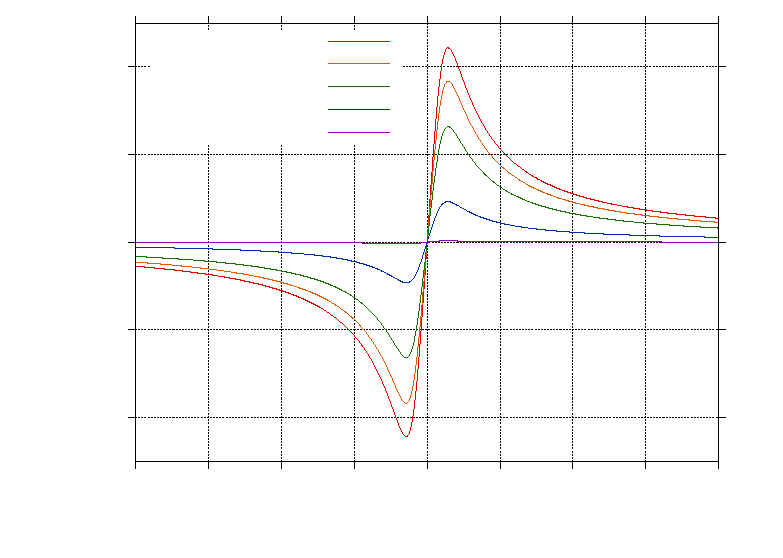
\includegraphics{Figures/DeltapwaveTnon0/kdepend}}%
    \gplfronttext
  \end{picture}%
\endgroup
  
\caption{The numerically calculated gap $\Delta_k$ is plotted as a function of $k$ for different temperatures. Parameters: $k_F a_B = k_F a_{BF} = 0.3, k_F l_t = 0.01, \frac{m_F}{m_B} = 0.8, \frac{n_B}{n_F^3} = 0.9$. }  
\label{fig.Deltakkdepend}  
\end{center}    
\end{figure}

\begin{figure} 
\begin{center}  
% GNUPLOT: LaTeX picture with Postscript
\begingroup
  \makeatletter
  \providecommand\color[2][]{%
    \GenericError{(gnuplot) \space\space\space\@spaces}{%
      Package color not loaded in conjunction with
      terminal option `colourtext'%
    }{See the gnuplot documentation for explanation.%
    }{Either use 'blacktext' in gnuplot or load the package
      color.sty in LaTeX.}%
    \renewcommand\color[2][]{}%
  }%
  \providecommand\includegraphics[2][]{%
    \GenericError{(gnuplot) \space\space\space\@spaces}{%
      Package graphicx or graphics not loaded%
    }{See the gnuplot documentation for explanation.%
    }{The gnuplot epslatex terminal needs graphicx.sty or graphics.sty.}%
    \renewcommand\includegraphics[2][]{}%
  }%
  \providecommand\rotatebox[2]{#2}%
  \@ifundefined{ifGPcolor}{%
    \newif\ifGPcolor
    \GPcolorfalse
  }{}%
  \@ifundefined{ifGPblacktext}{%
    \newif\ifGPblacktext
    \GPblacktexttrue
  }{}%
  % define a \g@addto@macro without @ in the name:
  \let\gplgaddtomacro\g@addto@macro
  % define empty templates for all commands taking text:
  \gdef\gplbacktext{}%
  \gdef\gplfronttext{}%
  \makeatother
  \ifGPblacktext
    % no textcolor at all
    \def\colorrgb#1{}%
    \def\colorgray#1{}%
  \else
    % gray or color?
    \ifGPcolor
      \def\colorrgb#1{\color[rgb]{#1}}%
      \def\colorgray#1{\color[gray]{#1}}%
      \expandafter\def\csname LTw\endcsname{\color{white}}%
      \expandafter\def\csname LTb\endcsname{\color{black}}%
      \expandafter\def\csname LTa\endcsname{\color{black}}%
      \expandafter\def\csname LT0\endcsname{\color[rgb]{1,0,0}}%
      \expandafter\def\csname LT1\endcsname{\color[rgb]{0,1,0}}%
      \expandafter\def\csname LT2\endcsname{\color[rgb]{0,0,1}}%
      \expandafter\def\csname LT3\endcsname{\color[rgb]{1,0,1}}%
      \expandafter\def\csname LT4\endcsname{\color[rgb]{0,1,1}}%
      \expandafter\def\csname LT5\endcsname{\color[rgb]{1,1,0}}%
      \expandafter\def\csname LT6\endcsname{\color[rgb]{0,0,0}}%
      \expandafter\def\csname LT7\endcsname{\color[rgb]{1,0.3,0}}%
      \expandafter\def\csname LT8\endcsname{\color[rgb]{0.5,0.5,0.5}}%
    \else
      % gray
      \def\colorrgb#1{\color{black}}%
      \def\colorgray#1{\color[gray]{#1}}%
      \expandafter\def\csname LTw\endcsname{\color{white}}%
      \expandafter\def\csname LTb\endcsname{\color{black}}%
      \expandafter\def\csname LTa\endcsname{\color{black}}%
      \expandafter\def\csname LT0\endcsname{\color{black}}%
      \expandafter\def\csname LT1\endcsname{\color{black}}%
      \expandafter\def\csname LT2\endcsname{\color{black}}%
      \expandafter\def\csname LT3\endcsname{\color{black}}%
      \expandafter\def\csname LT4\endcsname{\color{black}}%
      \expandafter\def\csname LT5\endcsname{\color{black}}%
      \expandafter\def\csname LT6\endcsname{\color{black}}%
      \expandafter\def\csname LT7\endcsname{\color{black}}%
      \expandafter\def\csname LT8\endcsname{\color{black}}%
    \fi
  \fi
    \setlength{\unitlength}{0.0500bp}%
    \ifx\gptboxheight\undefined%
      \newlength{\gptboxheight}%
      \newlength{\gptboxwidth}%
      \newsavebox{\gptboxtext}%
    \fi%
    \setlength{\fboxrule}{0.5pt}%
    \setlength{\fboxsep}{1pt}%
\begin{picture}(7200.00,5040.00)%
    \gplgaddtomacro\gplbacktext{%
      \csname LTb\endcsname%
      \put(1078,767){\makebox(0,0)[r]{\strut{}$0$}}%
      \csname LTb\endcsname%
      \put(1078,1819){\makebox(0,0)[r]{\strut{}$0.005$}}%
      \csname LTb\endcsname%
      \put(1078,2872){\makebox(0,0)[r]{\strut{}$0.01$}}%
      \csname LTb\endcsname%
      \put(1078,3924){\makebox(0,0)[r]{\strut{}$0.015$}}%
      \csname LTb\endcsname%
      \put(1078,4976){\makebox(0,0)[r]{\strut{}$0.02$}}%
      \csname LTb\endcsname%
      \put(1273,484){\makebox(0,0){\strut{}$0$}}%
      \csname LTb\endcsname%
      \put(2366,484){\makebox(0,0){\strut{}$0.002$}}%
      \csname LTb\endcsname%
      \put(3460,484){\makebox(0,0){\strut{}$0.004$}}%
      \csname LTb\endcsname%
      \put(4553,484){\makebox(0,0){\strut{}$0.006$}}%
      \csname LTb\endcsname%
      \put(5647,484){\makebox(0,0){\strut{}$0.008$}}%
      \csname LTb\endcsname%
      \put(6740,484){\makebox(0,0){\strut{}$0.01$}}%
    }%
    \gplgaddtomacro\gplfronttext{%
      \csname LTb\endcsname%
      \put(176,2871){\rotatebox{-270}{\makebox(0,0){\strut{}$Deltamax/eF$}}}%
      \put(4006,154){\makebox(0,0){\strut{}$T/TF$}}%
    }%
    \gplbacktext
    \put(0,0){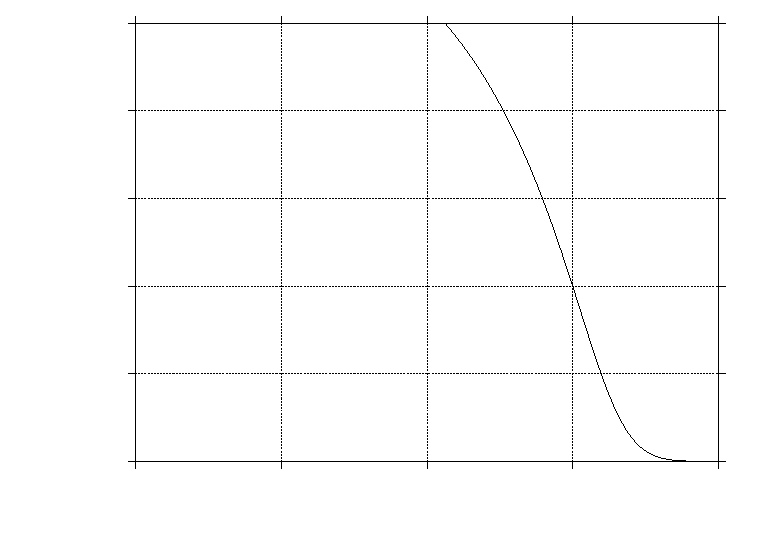
\includegraphics{Tdepend}}%
    \gplfronttext
  \end{picture}%
\endgroup
  
\caption{The numerically calculated temperature dependency of the maximum $\max_k[\Delta_k]$. Notice, that the critical temperature at which the gap becomes vanishing is $T_C \approx 0.14 T_F$, and that the gap is not monotonically decreasing, but a little lower at $T=0$ than in the interval $0<T/T_F<0.05$. Parameters: $k_F a_B = k_F a_{BF} = 0.3, k_F l_t = 0.01, \frac{m_F}{m_B} = 0.8, \frac{n_B}{n_F^3} = 0.9$. }  
\label{fig.maxkDeltakTdepend}  
\end{center}    
\end{figure}

It turns out, that this solution is essentially a $l_t \to 0$ limit. This is checked by taking $l_t$ a factor of 10 smaller and observing no difference. The divergence met in chapter \ref{Chapter3} is gone! It is further seen, that we can enhance the response (increase $\Delta_k$) by letting $a_B$ be significantly smaller than $a_{BF}$. However, we then come into trouble with the above assumptions about the chemical potential. We observe for the solution at hand, that the pairing potential is uneven in $k$ as already argued, and that it goes to 0 for $k/k_F \gg 1$. This decay does not however seem to be exponential, but rather of a power type. Further, from around $T/T_F = 0.006$ the maximum value of the gap $\max_k[\Delta_k]$ decreases monotonically to 0. The critical temperature is approximately $T_C/T_F = 0.136$ and the maximal gap size is $\max_{k,T}[\Delta_k(T)]/\epsilon_F = 0.222$, so $\frac{\max_{k,T}[\Delta_k(T)]}{k_B T_C} = \frac{0.222}{0.136} = 1.634$. This is not far from the BCS-value of the gap to critical temperature ratio: $1.765$ \cite{BruusFlensberg}. 